\documentclass{article}
\usepackage[margin=1in]{geometry}
\usepackage{enumitem}
\usepackage{titlesec}
\usepackage{xcolor}
\usepackage{fontspec}
\usepackage{setspace}
\usepackage{parskip}
\usepackage{graphicx}
\usepackage{fancyhdr}
\usepackage{tcolorbox}
\usepackage{array}
\usepackage{booktabs}
\usepackage{hyperref}

% Define custom colors
\definecolor{primarycolor}{RGB}{70, 130, 180} % Steel Blue
\definecolor{secondarycolor}{RGB}{245, 245, 245} % Light Grey
\definecolor{accentcolor}{RGB}{255, 140, 0} % Dark Orange

% Configure hyperref
\hypersetup{
    colorlinks=true,
    linkcolor=primarycolor,
    urlcolor=accentcolor,
    citecolor=primarycolor,
}

% Format section titles
\titleformat{\section}
  {\normalfont\Large\bfseries\color{primarycolor}}
  {\thesection.}{0.5em}{}[\titlerule]

% Set up fancy headers
\pagestyle{fancy}
\fancyhf{}
\fancyhead[L]{Team Oaklaura}
\fancyhead[R]{CS340 - Introduction to Databases, Spring 2025}
\fancyfoot[C]{\thepage}
\renewcommand{\headrulewidth}{1pt}
\renewcommand{\headrule}{\hbox to\headwidth{\color{primarycolor}\leaders\hrule height \headrulewidth\hfill}}

% Custom item formatting
\setlist[itemize]{leftmargin=*, label={\color{accentcolor}$\bullet$}}

\begin{document}

\begin{center}
\large\textcolor{primarycolor}{\textbf{Project Group \#1}}\\[0.3cm]
\large\textbf{Grant Wu and Jessica Ramirez}\\[0.3cm]
\huge\textbf{Project Step 1 - Database Design}\\[1.25cm]
\end{center}

\section{The Oaklaura Bike Cooperative}

\begin{tcolorbox}[colback=secondarycolor, colframe=primarycolor, arc=5mm]
\begingroup
\large
The Oaklaura Bike Cooperative is a non-profit organization that accepts donations of old or broken bicycles, refurbishes them, and then sells them at an affordable price. Due to limited funding, the co-op operates with a small team of employees and relies heavily on volunteers to assist with bicycle repairs. The co-op’s limited funding also requires they use a basic POS system that can only process one bike sale at a time, setting a limit of one bike per sales order.

\vspace{0.2cm}

Store Personnel consist of both volunteers and employees. Most volunteers are not experienced bike mechanics, so they often can't fully repair a bike during the few hours the co-op is open for volunteer work. To maintain continuity and organization, volunteers are expected to repair what they can during their shift and document their progress in a report. This allows the next volunteer and/or employee to review the logs and continue the work where the previous one left off. Once a volunteer believes a bike is fully repaired, a trained employee inspects it to ensure it meets safety standards before placing it on the sales floor.

\vspace{0.2cm}

Historically, the co-op tracked repair progress and sales using handwritten notecards stored in a filing cabinet. However, as the organization grows, this system has become increasingly difficult to manage. Implementing a database would be an ideal solution for organizing and sharing information between volunteers and employees about the status of each bicycle.

\endgroup
\end{tcolorbox}

\vspace{0.5cm}

\section{Database Schema}

\begin{tcolorbox}[colback=secondarycolor, colframe=primarycolor, title=\textbf{Bikes Table}]
Contains details on a particular bike within the co-op
\vspace{0.2cm}

\begin{itemize}
  \item \textbf{bikeID [PK]:} int, not NULL, auto\_increment
  \item \textbf{color:} enum('Black', 'White', 'Red', 'Blue', 'Green', 'Pink', 'Purple', 'Yellow', 'Orange', 'Silver', 'Other'), not NULL 
  \item \textbf{style:} enum('Mountain', 'Road', 'Fat', 'Hybrid', 'Enduro', 'BMX', 'Cruiser', 'Kids', 'Electric'), not NULL
  \item \textbf{brand:} varchar(45)
  \item \textbf{status:} enum('In Repair', 'Employee Review', 'For Sale', 'Sold'), not NULL
  \item \textbf{dateReceived:} date, not NULL
  \item \textbf{completed:} tinyint(default 0=false), not NULL
\end{itemize}
\vspace{0.2cm}

\textbf{Relationships:}
\vspace{0.2cm}
\begin{itemize}
  \item M:M relationship between Bikes and StorePersonnel is implemented with bikeID and personnelID as FK's within both RepairReports and within SalesReports.
  \item 1:1 relationship between Bikes and SalesReports is implemented by bikeID as a FK within SalesReports. \textit{Note that due to our outdated POS system, only one bike can be sold at a time (i.e. only one Bike instance per SalesReport instance).}
  \item 1:M relationship between Bikes and RepairReports is implemented with bikeID as a FK within RepairReports.
  \item 1:M relationship between Bikes and SalesReports is implemented with bikeID as a FK within SalesReports.
\end{itemize}
\end{tcolorbox}

\vspace{0.5cm}

\begin{tcolorbox}[colback=secondarycolor, colframe=primarycolor, title=\textbf{StorePersonnel Table}]
Holds information on store employees and volunteers
\vspace{0.2cm}

\begin{itemize}
  \item \textbf{personnelID [PK]:} int, not NULL, auto\_increment
  \item \textbf{firstName:} varchar(45) not NULL
  \item \textbf{lastName:} varchar(45) not NULL
  \item \textbf{phone:} varchar(20)
  \item \textbf{email:} varchar(100), not NULL, unique
  \item \textbf{role:} enum('Employee', 'Volunteer'), not NULL
\end{itemize}
\vspace{0.2cm}

\textbf{Relationships:}
\vspace{0.2cm}
\begin{itemize}
  \item M:M relationship between StorePersonnel and Bikes is implemented with bikeID and personnelID as FK's within both RepairReports and within SalesReports.
  \item 1:M relationship between StorePersonnel and RepairReports is implemented with personnelID as a FK within RepairReports.
  \item 1:M relationship between StorePersonnel and SalesReports is implemented with personnelID as a FK within SalesReports.
\end{itemize}
\end{tcolorbox}

\vspace{0.5cm}

\begin{tcolorbox}[colback=secondarycolor, colframe=primarycolor, title=\textbf{Customers Table}]
Holds customer information
\vspace{0.2cm}

\begin{itemize}
  \item \textbf{customerID [PK]:} int, not NULL, auto\_increment
  \item \textbf{firstName:} varchar(45) not NULL
  \item \textbf{lastName:} varchar(45) not NULL
  \item \textbf{phone:} varchar(20)
  \item \textbf{email:} varchar(100), not NULL, UNIQUE
\end{itemize}
\vspace{0.2cm}

\textbf{Relationships:}
\vspace{0.2cm}
\begin{itemize}
  \item 1:M relationship between Customers and SalesReports is implemented with customerID as a FK inside of SalesReports.
\end{itemize}
\end{tcolorbox}

\vspace{0.5cm}

\begin{tcolorbox}[colback=secondarycolor, colframe=primarycolor, title=\textbf{RepairReports Table}]
Holds repair information performed on a particular bikes (Bikes\_StorePersonnel Intersection Table that includes additional repair information)
\vspace{0.2cm}

\begin{itemize}
  \item \textbf{repairID [PK]:} int, not NULL, auto\_increment
  \item \textbf{personnelID [FK - StorePersonnel]:} int, not NULL
  \item \textbf{bikeID [FK - Bikes]:} int, not NULL
  \item \textbf{dateRepaired:} datetime, not NULL
  \item \textbf{hoursSpent:} decimal(4,2), not NULL
  \item \textbf{description:} varchar(255)
\end{itemize}
\vspace{0.2cm}

\textbf{Relationships:}
\vspace{0.2cm}
\begin{itemize}
  \item 1:M relationship between RepairReports and StorePersonnel is implemented with personnelID as a FK inside RepairReports.
  \item 1:M relationship between RepairReports and Bikes is implemented with bikeID as a FK inside RepairReports.
\end{itemize}
\end{tcolorbox}

\vspace{0.5cm}

\begin{tcolorbox}[colback=secondarycolor, colframe=primarycolor, title=\textbf{SalesReports Table}]
Holds information pertaining to the sale of a particular bike (Bikes\_StorePersonnel Intersection Table that includes additional sale information)
\vspace{0.2cm}

\begin{itemize}
  \item \textbf{salesID [PK]:} int, not NULL, auto\_increment
  \item \textbf{personnelID [FK - StorePersonnel]:} int, not NULL
  \item \textbf{bikeID [FK - Bikes]:} int, not NULL
  \item \textbf{customerID [FK - Customers]:} int, not NULL
  \item \textbf{dateSold:} date, not NULL
  \item \textbf{price:} decimal(5,2), not NULL
\end{itemize}
\vspace{0.2cm}

\textbf{Relationships:}
\vspace{0.2cm}
\begin{itemize}
  \item 1:1 relationship between Bikes and SalesReports is implemented by bikeID as a FK within SalesReports. \textit{Note that due to our outdated POS system, only one bike can be sold at a time (i.e. only one Bike instance per SalesReport instance).}
  \item 1:M relationship between SalesReports and StorePersonnel is implemented with personnelID as a FK within SalesReports.
  \item 1:M relationship between SalesReports and Customers is implemented with customerID as a FK within SalesReports.
\end{itemize}
\end{tcolorbox}

\vspace{0.5cm}

\section{Entity-Relationship Diagram}

\begin{tcolorbox}[colback=secondarycolor, colframe=primarycolor, arc=5mm]

\begin{center}
\vspace{0.5cm}
 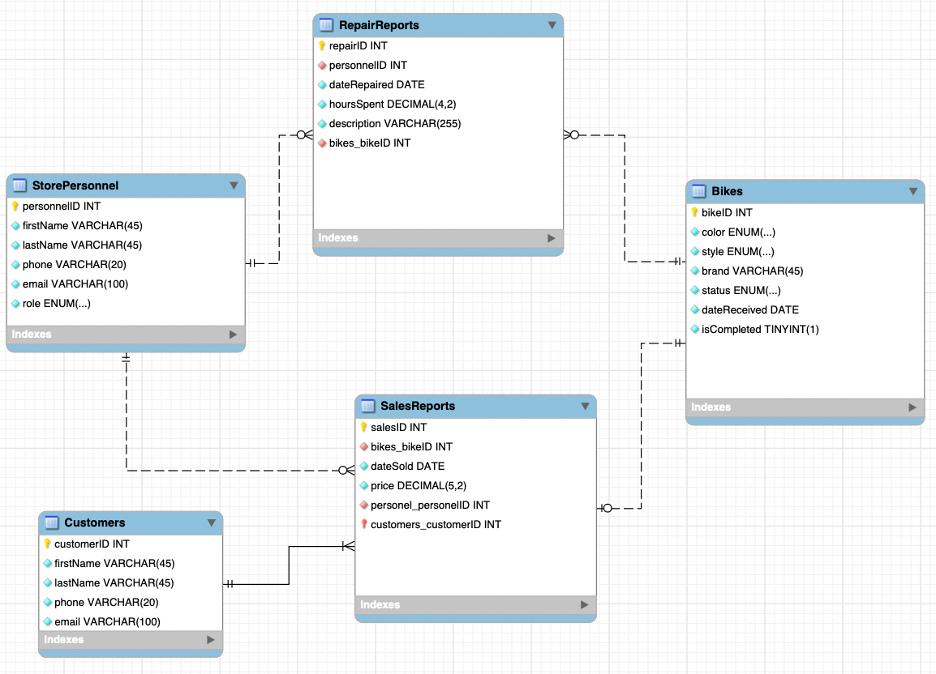
\includegraphics[width=0.9\textwidth]{ERD.png}
\end{center}
\end{tcolorbox}

\vspace{0.5cm}

\section{Citations}
\begin{tcolorbox}[colback=secondarycolor, colframe=primarycolor, arc=5mm]
\begin{itemize}
  \item Inspiration for the Bike Co-Op came from The Recyclery, a non-profit bike shop based out of Chicago, IL (last retrieved on 4/9/2025): \href{https://www.therecyclery.org/}{https://www.therecyclery.org/}
  
  \vspace{0.2cm}
  
  \item MySQL workbench was used to create the ERD diagram shown above.
  
  \vspace{0.2cm}
  
  \item The \LaTeX\ template used here was adapted from the Cleese-Assignment template v.2.0 (retrieved on 4/2/2025): \href{https://latextemplates.com/template/cleese-assignment}{https://latextemplates.com/template/cleese-assignment}
  
  \vspace{0.2cm}
  
  \item TeXShop was used for all \LaTeX\ related compilations.
  
  \vspace{0.2cm}
  
  \item All database and design related work is original.
\end{itemize}
\end{tcolorbox}

\end{document}